\section{A Semantic Wiki for Science}
\label{sec:science}

\begin{wrapfigure}{r}{4.2cm}
  \centering
  \vspace{-.9cm}
  \begin{tikzpicture}
    \node (s) at (0,0) {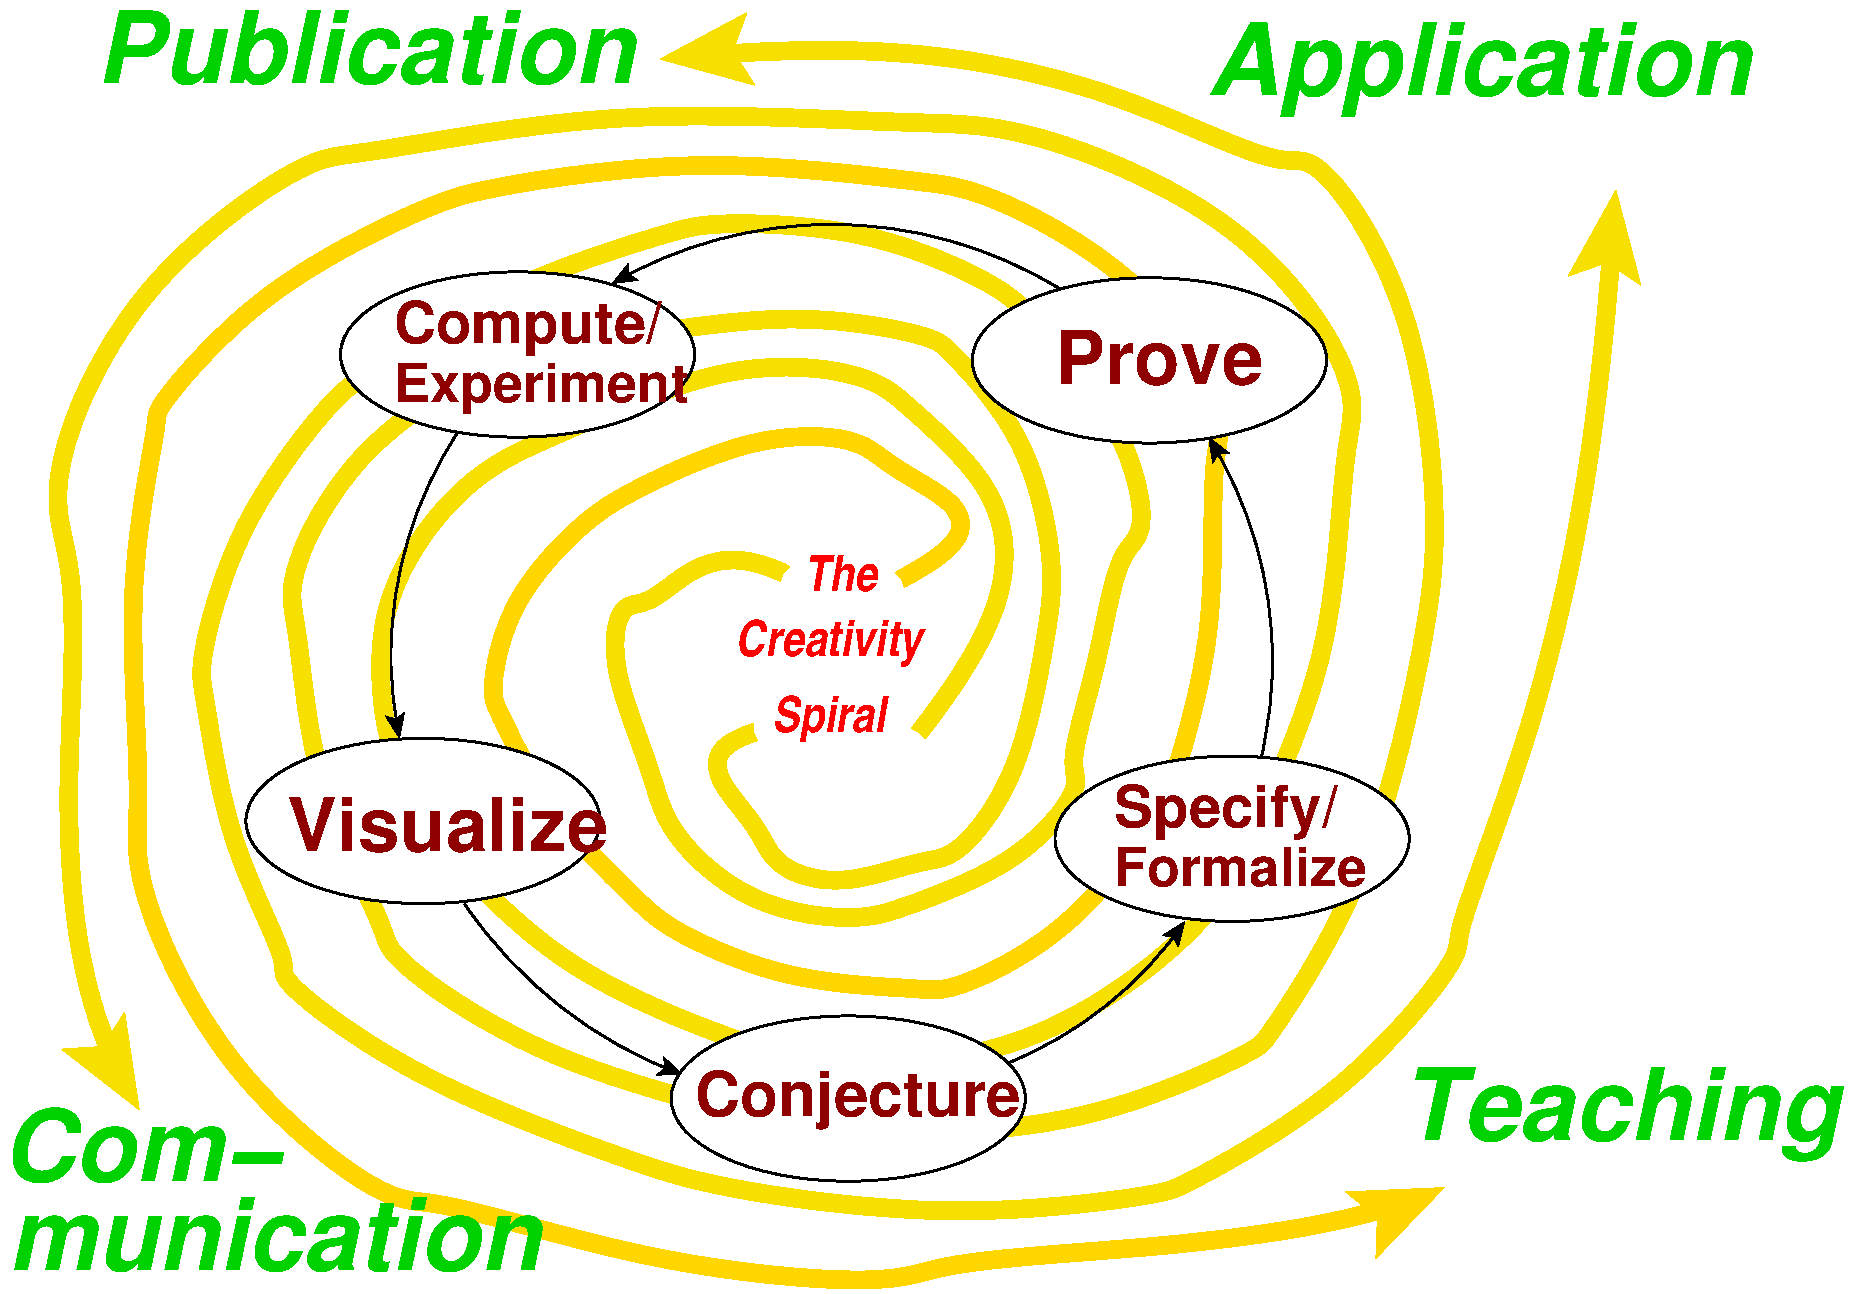
\includegraphics[width=4cm]{images/creativity-spiral}};
    \node at (s.south) {\scriptsize (B.\ Buchberger, 1995)};
  \end{tikzpicture}
  \vspace{-1.2cm}
\end{wrapfigure}
Documents are the most important medium in science, if we assume a broad definition of
``document'', including any materialized item of (scientific) knowledge.  Scientific
communication mainly consists of exchanging documents---from informal drafts circulating
inside a working group to published, well-structured books.  A great deal of scientific
work consists of collaboratively authoring these documents---taking down first hypotheses,
commenting on results of experiments or project steps, as well as structuring, annotating,
and re-organizing existing items of knowledge.  Tools that
\emph{understand} the knowledge contained in scientific documents are desirable for
editing such documents.  One approach towards this is writing scientific documents in a
semantic markup language with an editor that knows the structures available in this
language.

Besides generic approaches like SALT\cite{Groza:SALT07}, semantic markup has
been most deeply investigated in the specific domain of mathematics with its
``long tradition in the pursuit of conceptual clarity and representational
rigor''\cite{Kohlhase:omdoc1.2}, resulting in languages like
MathML\cite{CarlisleEd:MathML07}, OpenMath\cite{BusCapCar:2oms04}, and
OMDoc\cite{Kohlhase:omdoc1.2}.  OMDoc is a language that employs Content MathML,
the structure-oriented sublanguage of MathML, or OpenMath for structurally
representing mathematical \emph{objects} (symbols, numbers, equations, etc.) and
adds two layers on top of that: Objects or informal text can be annotated as
mathematical \emph{statements} (symbol declarations, definitions, axioms,
theorems, proofs, examples, etc.), and collections of interrelated statements
are grouped into \emph{theories}.

With SWiM, a semantic wiki for mathematical knowledge management (see
section~\ref{sec:swim}), we have investigated collaborative editing of OMDoc
documents.  It has turned out that a wiki is a suitable tool for supporting the
workflow of incremental formalization inherent to scientific writing.  But wikis
have not only shown to be appropriate for \emph{writing}, but there are also
many success stories from project management, e.\,g.\ in corporate
settings\cite{leuf01:wikiway,wikinomics}.  Thus, we are interested in applying
our technologies to scientific knowledge engineering projects.

%%% Local Variables: 
%%% mode: latex
%%% TeX-master: "flyspeck-wiki-eswc08"
%%% End: 
